\section{Coleta de Dados}
A coleta será feita utilizando a API publica do twitter, o link para a documentção é \url{https://developer.twitter.com/en/docs}. Será trabalhado no projeto duas entidades: Tweet e Usuário. O tweet é a entidade que representa a publicação do usuário, enquanto o usuário contém informações necessárias sobre o seu perfil.

Para que seja possível acessar a API é necessário criar uma conta de desenvolvimento e gerar o \textit{token} de acesso através do link \url{https://apps.twitter.com/app/new}. Com a chave em mãos é possível replicar o arquivo /collector/client/.env\_sample dentro do projeto Dumont para /collector/client/.env, e conforme demonstrado na figura \ref{fig:twitteropts}, completar os campos necessários.

\begin{figure}
    \centering
    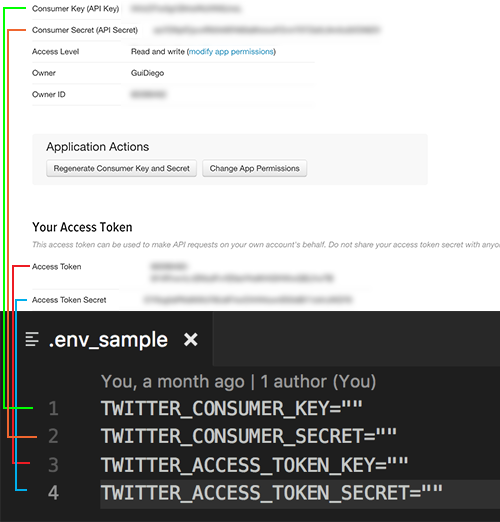
\includegraphics[width=.8\textwidth]{imagens/twitteropts.png}
    \caption{Diagrama demonstrando o funcionamento da ferramenta APPA}
    \label{fig:twitteropts}
\end{figure}

Para rodar basta executar o comando \textit{docker run -it --rm --name dumont -v \$"PWD":/usr/src/app -w /usr/src/app node:9 node collector/twitter.js}, e verá a saída de dados.

Uma vez configurado o coletor, ainda é necessário entender e configurar as outras tarefas para que o APPA funcione apropriadamente, logo, é necessário entender como essas entidades ficarão no final e quais as tarefas que realização essa manipulação.

